%%%% A summary of basic Markov decision theory.

% Plain and simple
\documentclass{article}

% Format and figure stuff
\usepackage{geometry}
\usepackage{graphicx}
\usepackage{float}
\usepackage[usenames, dvipsnames]{color}

% Text stuff
\usepackage{tikzsymbols}

% Math stuff
\usepackage{mathtools}
\usepackage{mathrsfs}
\usepackage{amsmath}
\usepackage{amssymb}
\usepackage{cancel}
\usepackage{xfrac}
\usepackage{bm}

% Code stuff
\usepackage{listings}
\usepackage{hyperref}

% Page layout
\geometry{top=1in,bottom=1in}
\hyphenpenalty = 10000
\setlength\parindent{0pt}
\setlength{\jot}{10pt}

% Hyperlink format
\hypersetup{colorlinks=true,
            linkcolor=blue,
            filecolor=magenta,
            urlcolor=blue}

% Tab command
\newcommand\tab[1][1cm]{\hspace*{#1}}

% Line command
\newcommand\myline{\noindent\makebox[\linewidth]{\rule{\paperwidth - 2in}{0.4pt}}}

% Code font
\def\code#1{\texttt{#1}}

% Quick colors
\definecolor{stateblue}{rgb}{0, 0, 0.75}
\definecolor{darkgreen}{rgb}{0, 0.5, 0}
\definecolor{orange}{RGB}{180, 60, 0}
\definecolor{purple}{RGB}{200, 0, 200}
\def\green#1{\textcolor{darkgreen}{#1}}
\def\red#1{\textcolor{red}{#1}}
\def\blue#1{\textcolor{stateblue}{#1}}
\def\orange#1{\textcolor{orange}{#1}}
\def\purple#1{\textcolor{purple}{#1}}
\def\black#1{\textcolor{black}{#1}}

% Coordinate system notation
\def\cs#1#2%
  {\mathop{}%
   \mathopen{\vphantom{#2}}^{#1}%
   \kern-\scriptspace%
   #2}

% Custom math symbols - linear algebra
\DeclareMathOperator*{\tr}{\intercal}
\DeclareMathOperator*{\zero}{\underline{0}}
\DeclareMathOperator*{\eye}{\underline{1}}
\newcommand\inv[1]{#1\raisebox{1.15ex}{$\scriptscriptstyle-\!1$}}
\newcommand\pinv[1]{#1\raisebox{1.15ex}{$\scriptscriptstyle\dist\!1$}}

% Custom math symbols - probability
\DeclareMathOperator*{\E}{E}
\DeclareMathOperator*{\cov}{cov}
\DeclareMathOperator*{\dist}{\sim}
\DeclareMathOperator*{\argmin}{arg\,min}
\DeclareMathOperator*{\argmax}{arg\,max}


\begin{document}

%%%%%%%%%%%%%%%%%%%%%%%%%%%%%%%%%%%%%%%%%%%%%%%%% TITLE

\title{\textbf{Markov Decision Processes}\\ \large{A Reasonably Precise Summary}\vspace{-6ex}}
\author{\vspace{-5ex}}
\date{\small{Jason Nezvadovitz -- February 2020}}
\maketitle

%%%%%%%%%%%%%%%%%%%%%%%%%%%%%%%%%%%%%%%%%%%%%%%%% BODY

The purpose of this document is to provide a written, mathematically precise summary of basic Markov decision theory for review. The focus is on axiomatic clarity rather than intuition. I encourage the reader to try explaining each statement intuitively while verifying its consistency.

\vspace{0.2in}
\hrule
\vspace{0.2in}

Declare ``time'': a countable set $\mathbb{T} \coloneqq \{0, 1, 2, \cdots, n\}$ for some potentially infinite ``horizon'' $n$.\\
Denote a generic element as $t \in \mathbb{T}$.\\

In the most general setting, time can be continuous (uncountable), but we will restrict ourselves to discrete time here to avoid the complications of stochastic calculus.\\

Declare the ``state space'': a set $\mathbb{S}$ of any cardinality. Could be $\mathbb{R}^2$, \{\Smiley,\Cooley,\Winkey\}, whatever.\\
Denote a generic element as $s \in \mathbb{S}$.\\

Declare the ``action space'': a set $\mathbb{A}$ of any cardinality. No restrictions.\\
Denote a generic element as $a \in \mathbb{A}$.\\

We will now build a standard \href{https://en.wikipedia.org/wiki/Probability_space}{probability space}, $\boldsymbol{(}\Omega, \mathcal{F}, P\boldsymbol{)}$.\\

Let the sample space be \ $\Omega \coloneqq \mathbb{S}^{n+1} \times \mathbb{A}^n \times \mathbb{R}^n$.\\
An individual sample $\omega \in \Omega$ is called a ``trajectory.''\\

Each trajectory consists of an ``initial condition'' $s_0$, and $n$ triplets of the form $(a_t, s_{t+1}, r_{t+1})$ called ``transitions,'' where the $r \in \mathbb{R}$ are called ``rewards.'' I.e.,
\begin{equation*}
\omega \coloneqq \{s_0, (a_0, s_1, r_1), (a_1, s_2, r_2), \cdots, (a_{n-1}, s_{n}, r_n)\}
\end{equation*}

The event set $\mathcal{F}$ is, as usual, the product sigma-algebra of $\Omega$, using the Borel sigma-algebra for uncountable sets and the power-set sigma-algebra for countable sets.\\

The probability measure $P$ is, as usual, defined in terms of the probability distribution $p$ by sums,
\begin{equation*}
P(B) \coloneqq \int_B p(\omega)\, d\omega\ \ \forall B \in \mathcal{F},\ \ \text{where}\ \ p(\omega)\geq0\ \ \text{and}\ \ \int_\Omega p(\omega)\,d\omega = 1
\end{equation*}

We declare $p$ to have ``Markovian'' structure, i.e. the following factorization:
\begin{align*}
p(\omega) &= p(s_0, a_0, s_1, r_1, a_1, s_2, r_2, \cdots, a_{n-1}, s_{n}, r_n)\\
&\stackrel{\text{markov}}{\coloneqq}\ p(s_0) \prod_{t=0}^{n-1} \red{p(a_t|s_t)}\blue{p(s_{t+1}|s_t,a_t)}\green{p(r_{t+1}|s_t,a_t,s_{t+1})}
\end{align*}

where we are using the usual overloaded notation for marginal and conditional distributions,\\
\begin{equation*}
p(x) \coloneqq \int p(x,y)\,dy\ \ \ \text{and}\ \ \ p(x|y) \coloneqq \frac{p(x,y)}{p(y)}
\end{equation*}

Practically speaking, the Markov property allows us to completely define high-dimensional trajectory probability densities $p(\omega)$ by specifying just the following lower-dimensional distributions:
\begin{itemize}
  \item The ``initial condition'' $p(s_0)$
  \item The ``\red{policies}'' $p(a_t|s_t)\ \forall t$
  \item The ``\blue{dynamics}'' $p(s_{t+1}|s_t,a_t)\ \forall t$
  \item The ``\green{rewards}'' $p(r_{t+1}|s_t,a_t,s_{t+1})\ \forall t$
\end{itemize}

If, for example, the expression of $p(a_t|s_t)$ does not depend explicitly on the time index $t$, then we say there is just one ``policy'' (nonplural) and that it is ``time-invariant.'' It is often the case that all of the above are time-invariant, and so we really only have one unique policy, one unique dynamic, and one unique reward distribution that are just replicated $n$-times in the factorization of $p(\omega)$.\\

Also, whenever a distribution's form is that of a Dirac/Kronecker-delta, we call it ``deterministic'' instead of ``stochastic.'' It is common for both the policies and rewards to be deterministic. In fact, the reward distribution is often deterministic, time-invariant, and even independent of $s_{t+1}$, meaning that it can be fully specified by a single function $\bar{r}:\mathbb{S}\times\mathbb{A} \to \mathbb{R}$ through,
\begin{equation*}
p(r_{t+1}|s_t,a_t,s_{t+1}) = \delta\big{(}r_{t+1} - \bar{r}(s_t, a_t)\big{)} \tag{common}
\end{equation*}

Anyway, the Markov property implies many strong conditional independence statements. E.g.,
\begin{equation*}
p(s_{t+1}|s_t,a_t,s_{t-1},a_{t-1},r_{t-1},s_{t-2},a_{t-2},r_{t-2},\cdots) = p(s_{t+1}|s_t,a_t)
\end{equation*}

These relationships can be depicted succinctly via a \href{https://en.wikipedia.org/wiki/Bayesian_network}{Bayesian graph} over the convenience random variables \ ${s_t}(\omega) \coloneqq s_t$, \ ${a_t}(\omega) \coloneqq a_t$, \ and \ ${r_t}(\omega) \coloneqq r_t$.
\begin{center}
  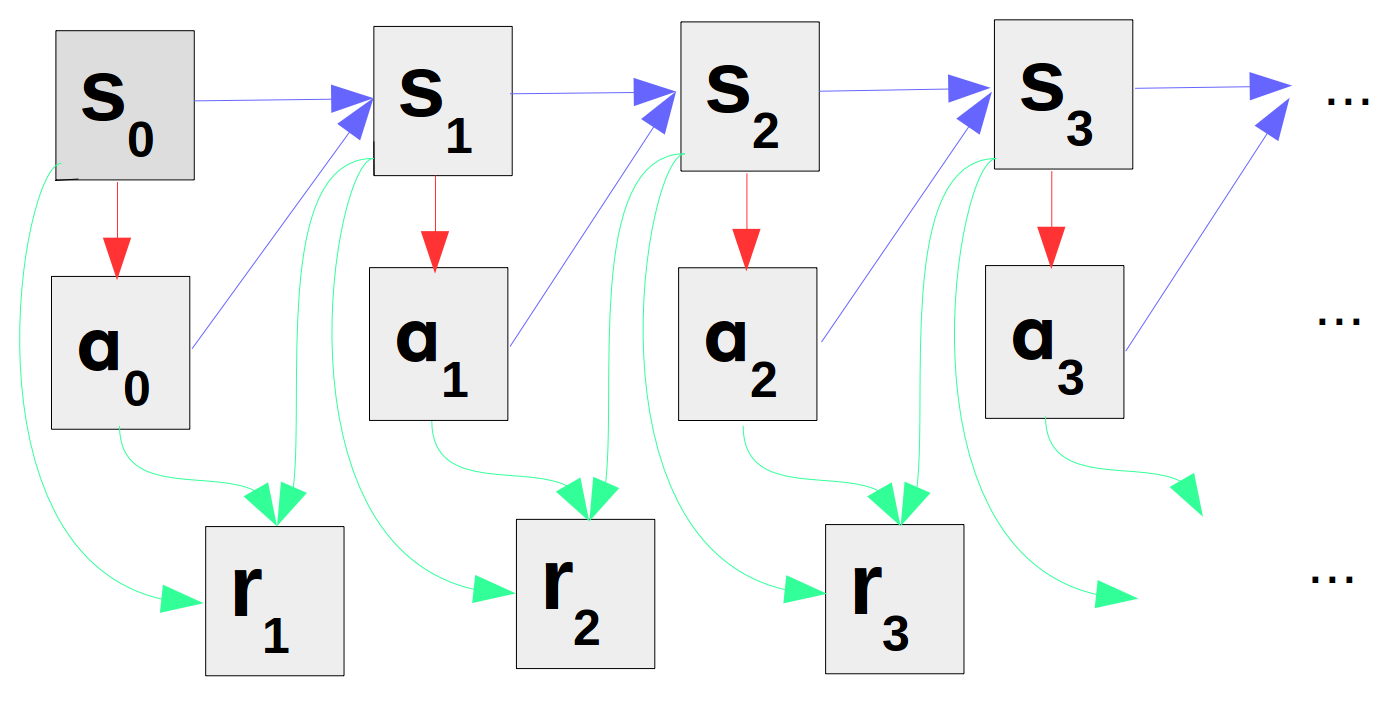
\includegraphics[width=\linewidth-1.5in]{include/bayesian_graph.png}
\end{center}

This temporally ``chained'' structure models the idea that ``given the present, the future is independent of the past'' and constitutes the entirety of a ``Markov decision process'' (MDP). Specifically, if we define the random variable $\omega_t$ to be the elements of a trajectory for times $\tau \geq t$ (``the future''),
\begin{equation*}
\omega_t \coloneqq \{s_t, (a_t, s_{t+1}, r_{t+1}), (a_{t+1}, s_{t+2}, r_{t+2}), \cdots, (a_{n-1}, s_{n}, r_n)\} \ \in \ \Omega_t \coloneqq \mathbb{S}^{n-t+1} \times \mathbb{A}^{n-t} \times \mathbb{R}^{n-t}
\end{equation*}

we see from the Bayesian graph that $\omega_t$ is disconnected from ``the past'' by conditioning on $s_t$,
\begin{equation*}
p(\omega_t|s_t) = \cancel{\frac{p(s_t)}{p(s_t)}}\prod_{\tau=t}^{n-1} p(a_\tau|s_\tau)p(s_{\tau+1}|s_\tau,a_\tau)p(r_{\tau+1}|s_\tau,a_\tau,s_{\tau+1})
\end{equation*}

We now define the ``total (discounted) reward from $t$'' to be a random variable that assesses the goodness of a sample of our MDP starting from time $t$ by summing up the remaining rewards,
\begin{align*}
G_t(\omega_t) &\coloneqq r_{t+1} + \gamma r_{t+2} + \gamma^2 r_{t+3} + \cdots + \gamma^{n-t-1} r_n\\
&= \sum_{\tau=t}^{n-1} \gamma^{\tau-t} r_{\tau+1}
\end{align*}

where $\gamma \in [0,1]$ is called the ``discount factor,'' used both to enforce the convergence of this sum (if $n \to \infty$) and to express that future rewards are less valuable than sooner rewards.\\

Total reward provokes an optimization problem: we want to choose the best possible policy distribution $p(a_t|s_t)$. To clarify, the ``decision'' in ``Markov decision process'' is really deciding the distribution from which actions will be sampled (the policy). If the policy depends only on time (ignoring the actual value of $s_t$) we call it ``open-loop'' or a ``plan,'' while if it depends on $s_t$ in any way we call it ``closed-loop.'' If the policy is deterministic and time-invariant, then it can be fully specified by a single function $\mathbb{S} \mapsto \mathbb{A}$ that is interpreted classically as a decision-making rule.\\

We will denote our choice as $\pi(a_t|s_t)$, and to emphasize that we have plugged-in our choice, we will use $\pi$ as a subscript on probability densities and statistics. For example,
\begin{equation*}
p_{\orange{\pi}}(\omega) \coloneqq p(\omega)\Big{|}_{p(a_t|s_t) = \orange{\pi(a_t|s_t)}} = p(s_0) \prod_{t=0}^{n-1} \orange{\pi(a_t|s_t)}p(s_{t+1}|s_t,a_t)p(r_{t+1}|s_t,a_t,s_{t+1})
\end{equation*}

But what does ``best'' mean with respect to a random variable like $G_t$? We choose to optimize a statistic of $G_t$. Namely, a conditional expectation called the ``value-function,''
\begin{align*}
V_\pi(s_t) &\coloneqq E_\pi(G_t | s_t)\\
&= \int_{\Omega_t} G_t(\omega_t) p_\pi(\omega_t|s_t)\,d\omega_t\\
&= \int_{\Omega_t} \sum_{\tau=t}^{n-1} \Big{(}\gamma^{\tau-t} r_{\tau+1}\Big{)} \prod_{\tau=t}^{n-1} \Big{(}\pi(a_\tau|s_\tau)p(s_{\tau+1}|s_\tau,a_\tau)p(r_{\tau+1}|s_\tau,a_\tau,s_{\tau+1})\Big{)} \,d\omega_t
\end{align*}

So $V_\pi(s_t)$ is the expected total reward acquired for starting from state $s$ at time $t$ and acting according to policy $\pi$. Our objective then is to find the optimal policy $\pi^*$ that satisfies,
\begin{equation*}
V_{\pi^*}(s_t) \geq V_{\pi}(s_t)\ \forall s_t
\end{equation*}

There is a necessary and sufficient condition for $\pi^*$ known as the ``dynamic programming principle'':
\begin{quote}
``An optimal policy has the property that, whatever the initial state and initial action are, the remaining actions must constitute an optimal policy with regard to the state resulting from the first action.'' (Bellman, 1957, Chapter III.3)
\end{quote}

This follows directly from the Markov property: given that the process is now in state $s_{t+1}$, the future of the process is independent of how it got there (i.e. the transition from $s_t$ using $a_t$). Therefore, if we can predict the optimal outcome from any $s_{t+1}$, we can determine $\pi^*(a_t|s_t)$ by optimizing just the expected immediate reward plus our prediction for the states we might transition to (discounted by $\gamma$ since it's future reward). Said mathematically,
\begin{gather*}
\pi^*(a_t|s_t) = \delta\big{(}a_t\ ;\ \bar{\pi}^*(s_t)\big{)}\\
\bar{\pi}^*(s_t) = \argmax_{a_t} E\big{(}r_{t+1} + \gamma V_{\pi^*}(s_{t+1}) | s_t, a_t\big{)}
\end{gather*}

However, this only gives us $\pi^*$ in terms of $V_{\pi^*}$ which we still don't know. To resolve this, consider the following recursion satisfied by the total reward,
\begin{align*}
G_t &= r_{t+1} + \gamma \big{(}r_{t+2} + \gamma r_{t+3} + \cdots + \gamma^{n-t-2} r_n\big{)}\\
&= r_{t+1} + \gamma G_{t+1}
\end{align*}

and the following properties of expectation for any random variables $x$, $y$, and $z$,
\begin{align*}
E(\alpha x + \beta y) &= \alpha E(x) + \beta E(y)\\
E(x | z) &= E\big{(}E(x | y, z) | z\big{)}
\end{align*}

It follows that any value-function also satisfies a recursion,
\begin{align*}
V_\pi(s_t) &= E_\pi(r_{t+1} + \gamma G_{t+1} | s_t)\\
&= E_\pi(r_{t+1}|s_t) + \gamma E_\pi(G_{t+1} | s_t)\\
&= E_\pi(r_{t+1}|s_t) + \gamma E_\pi\big{(}E_\pi(G_{t+1}|s_{t+1},s_t) | s_t\big{)}\\
&= E_\pi(r_{t+1}|s_t) + \gamma E_\pi\big{(}V_{\pi}(s_{t+1}) | s_t\big{)}\\
&= E_\pi\big{(}r_{t+1} + \gamma V_{\pi}(s_{t+1}) | s_t\big{)}
\end{align*}

And, since there is no more reward to be collected after time $n$, we have a boundary condition,
\begin{equation*}
V_{\pi}(s_n) = 0
\end{equation*}

Combining this recursion with the dynamic programming principle, we have the ``Bellman equation'':
\begin{equation*}
V^*(s_t) = \max_{a_t} E\big{(}r_{t+1} + \gamma V^*(s_{t+1}) | s_t, a_t\big{)}
\end{equation*}

with the shorthand $V^* \coloneqq V_{\pi^*}$. If we can solve the Bellman equation for $V^*$, then, as we saw before, $\pi^*$ can be constructed as the deterministic policy that always selects the $\argmax$ of the right-hand-side. Thus, a solution to the Bellman equation constitutes a solution to our MDP.\\

It is worth noting that the general value-function recursion is useful for more than just deriving the Bellman equation. It lets us compute the value-function associated with any policy, which can be useful when comparing candidate policies if the Bellman equation is too difficult to solve directly. The general value-function recursion doesn't involve the difficult maximization present in the Bellman equation and is even linear in the unknown $V_\pi$.\\

The expectations in these equations pack away a lot of computation, though they're not as intense as the expectation in the direct expression of $E_\pi(G_t|s_t)$, because the arguments of these expectations depend only on a single transition, not a whole trajectory, so we only need,
\begin{equation*}
p_\pi(a_t, s_{t+1}, r_{t+1}|s_t) = \orange{\pi(a_t|s_t)} \blue{p(s_{t+1}|s_t,a_t)} \green{p(r_{t+1}|s_t,a_t,s_{t+1})}
\end{equation*}

to express the general value-function recursion as,
\begin{align*}
V_\pi(s_t) &= E_\pi\big{(}r_{t+1} + \gamma V_{\pi}(s_{t+1}) | s_t\big{)}\\
&= \orange{\int_{\mathbb{A}} \pi(a_t|s_t) \blue{\int_{\mathbb{S}} p(s_{t+1}|s_t,a_t) \Big{(}\green{\int_{\mathbb{R}}p(r_{t+1}|s_t,a_t,s_{t+1}) r_{t+1} \,dr_{t+1}} + \gamma V_{\pi}(s_{t+1}) \Big{)}\,ds_{t+1}}\,da_t}
\end{align*}

and similarly express the Bellman equation as,
\begin{align*}
V^*(s_t) &= \max_{a_t} E\big{(}r_{t+1} + \gamma V^*(s_{t+1}) | s_t, a_t\big{)}\\
&= \orange{\max_{a_t} \blue{\int_{\mathbb{S}} p(s_{t+1}|s_t,a_t) \Big{(}\green{\int_{\mathbb{R}} p(r_{t+1}|s_t,a_t,s_{t+1})r_{t+1} \,dr_{t+1}} + \gamma V^*(s_{t+1}) \Big{)}\,ds_{t+1}}}
\end{align*}

This is the most general case for a (vanilla) MDP, but there are many very common situations that simplify things. For example, if the reward is deterministic and independent of $s_{t+1}$, it can be pulled out of the $\mathbb{R}$ and $\mathbb{S}$ integrations to write the Bellman equation as,
\begin{equation*}
V^*(s_t) = \max_{a_t} \big{(} \bar{r}(s_t, a_t) + \gamma T_{a_t} V^*(s_t) \big{)} \tag{common}
\end{equation*}

with the linear ``transition operator'' defined as,
\begin{align*}
T_{a_t} f(s_t) &\coloneqq E\big{(}f(s_{t+1})|s_t,a_t\big{)}\ \ \ \ \forall f : \mathbb{S} \times \mathbb{T} \to \mathbb{R}\\
&= \int_{\mathbb{S}}p(s_{t+1}|s_t,a_t)f(s_{t+1})\,ds_{t+1}
\end{align*}

Furthermore, if the MDP is time-invariant, infinite-horizon, and has finite state and action spaces, the above reduces to the form that is often presented first in introductory texts,
\begin{equation*}
V^*(s) = \max_{a} \Big{(} \bar{r}(s, a) + \gamma \sum_{s' \in \mathbb{S}} p(s'|s,a) V^*(s') \Big{)} \tag{common}
\end{equation*}

which can be readily implemented as matrix operations on the value-function as a single finite vector. It is also worth noting that if the dynamics are deterministic, the sum on the right reduces to a simple evaluation of $V^*$ at the state $s'$ deterministically transitioned to under action $a$.

\vspace{5ex}\hrule\vspace{2ex}

Next up:\\
- Using the Bellman equation directly (2d stochastic robber problem example, LQR example)\\
- Value iteration (contraction mapping, fixed-point iteration, small S example, markov diagrams)\\
- Q-learning (k-step value-functions, transition monte carlo, same small S example)\\
- Approximation (linear basis, deep nets, experience replay, S vs V smoothness, large S example)\\
- Policy gradient (analytical derivative, trajectory monte carlo)\\
- Allude further topics (POMDP / HMM, game theory / multiagent)

%%%%%%%%%%%%%%%%%%%%%%%%%%%%%%%%%%%%%%%%%%%%%%%%%

\end{document}
